% Chapter Template

\chapter{Ensayos y resultados} % Main chapter title
En esta sección se presentan los resultados obtenidos del desarrollo de hardware y software. Se analiza el cumplimiento de requisitos de desempeño impuestos por el cliente a trav\'{e}s de ensayos de laboratorio y finalmente, se exponen resultados de ensayos \textit{end to end} con la red LoRaWAN y un banco de prueba.\\
\label{Chapter4} % Change X to a consecutive number; for referencing this chapter elsewhere, use \ref{ChapterX}
%----------------------------------------------------------------------------------------
%	SECTION 1
%----------------------------------------------------------------------------------------
\section{Circuito impreso desarrollado}
\label{sec:pruebasHW}
Gracias al desarrollo temprano de la primera placa prototipo presentada en la figura \ref{fig:placaprototipo}, se realizaron las validaciones en el diseño de circuitos y selección de componentes para las diferentes etapas del hardware presentadas en la sección \ref{seccion_hardware}.\\
% TODO: \usepackage{graphicx} required
\begin{figure}[h]
	\centering
	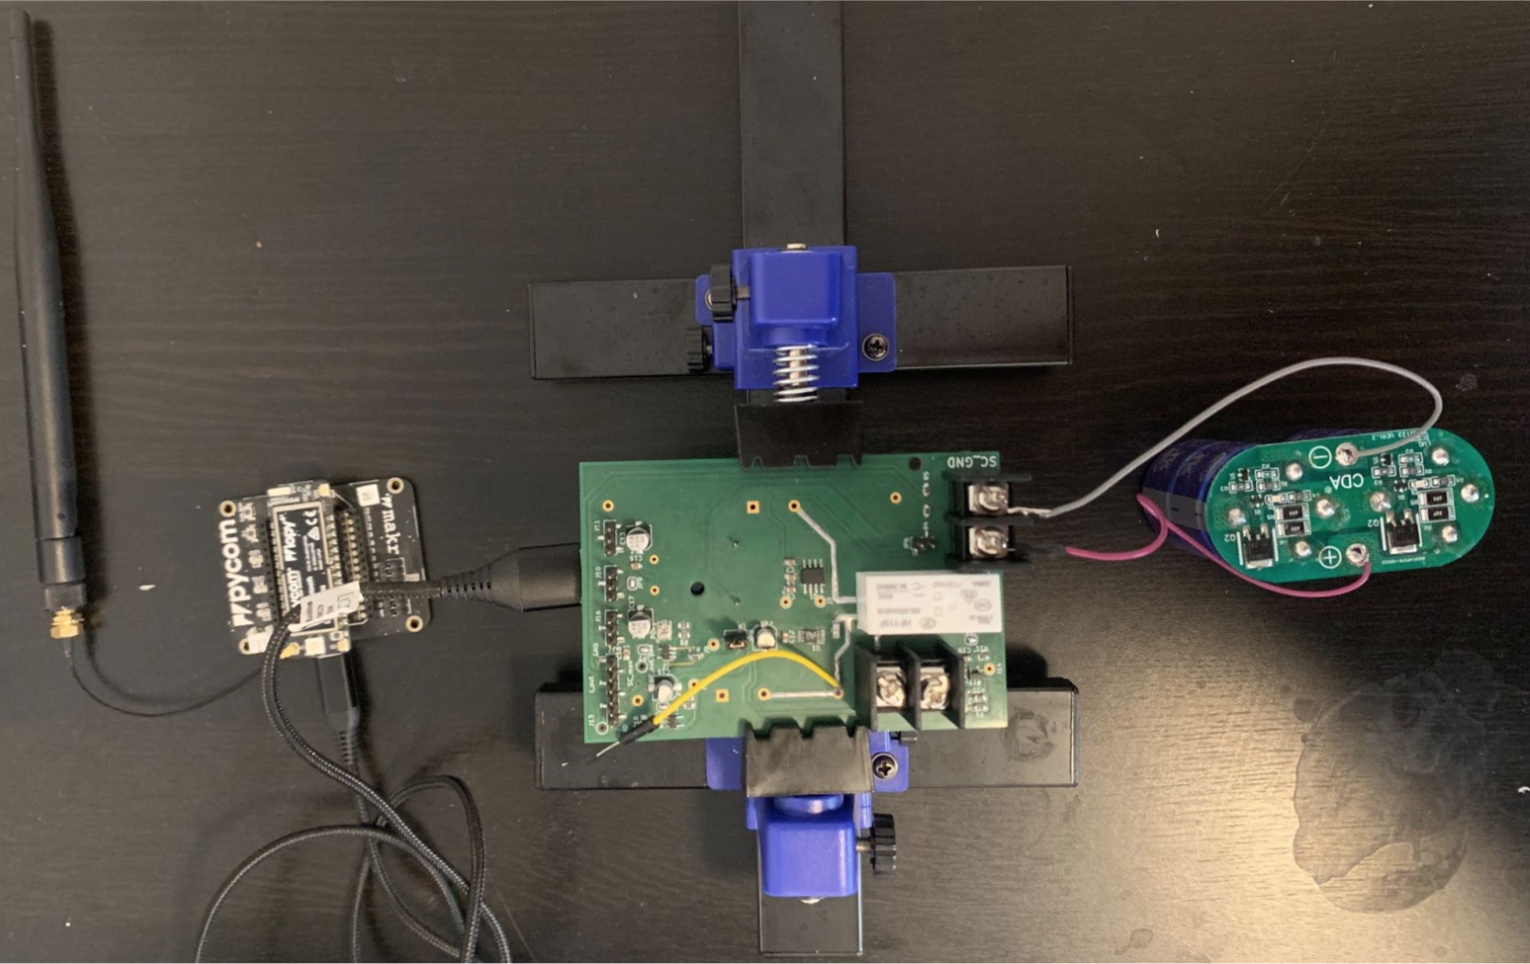
\includegraphics[width=1.0\linewidth]{Figures/placa_prototipo}
	\caption{Placa prototipo desarrollada para validación de diseños.}
	\label{fig:placaprototipo}
\end{figure}\\
Al disponer de una placa con la mayoría de las etapas ya montadas, soldadas y depuradas, se pudieron evitar fallas eléctricas tales como falsos contactos que ocurrieron al usar protoboards.\\
Una vez validados los diseños, se desarrolló la placa final presentada en las figuras \ref{fig:pcbfinaltop} y \ref{fig:pcbfinabottom}. Esta, a diferencia de la primera versi\'{o}n, integra todas las etapas en un único circuito impreso.\\
% TODO: \usepackage{graphicx} required
\begin{figure}[h!]
	\centering
	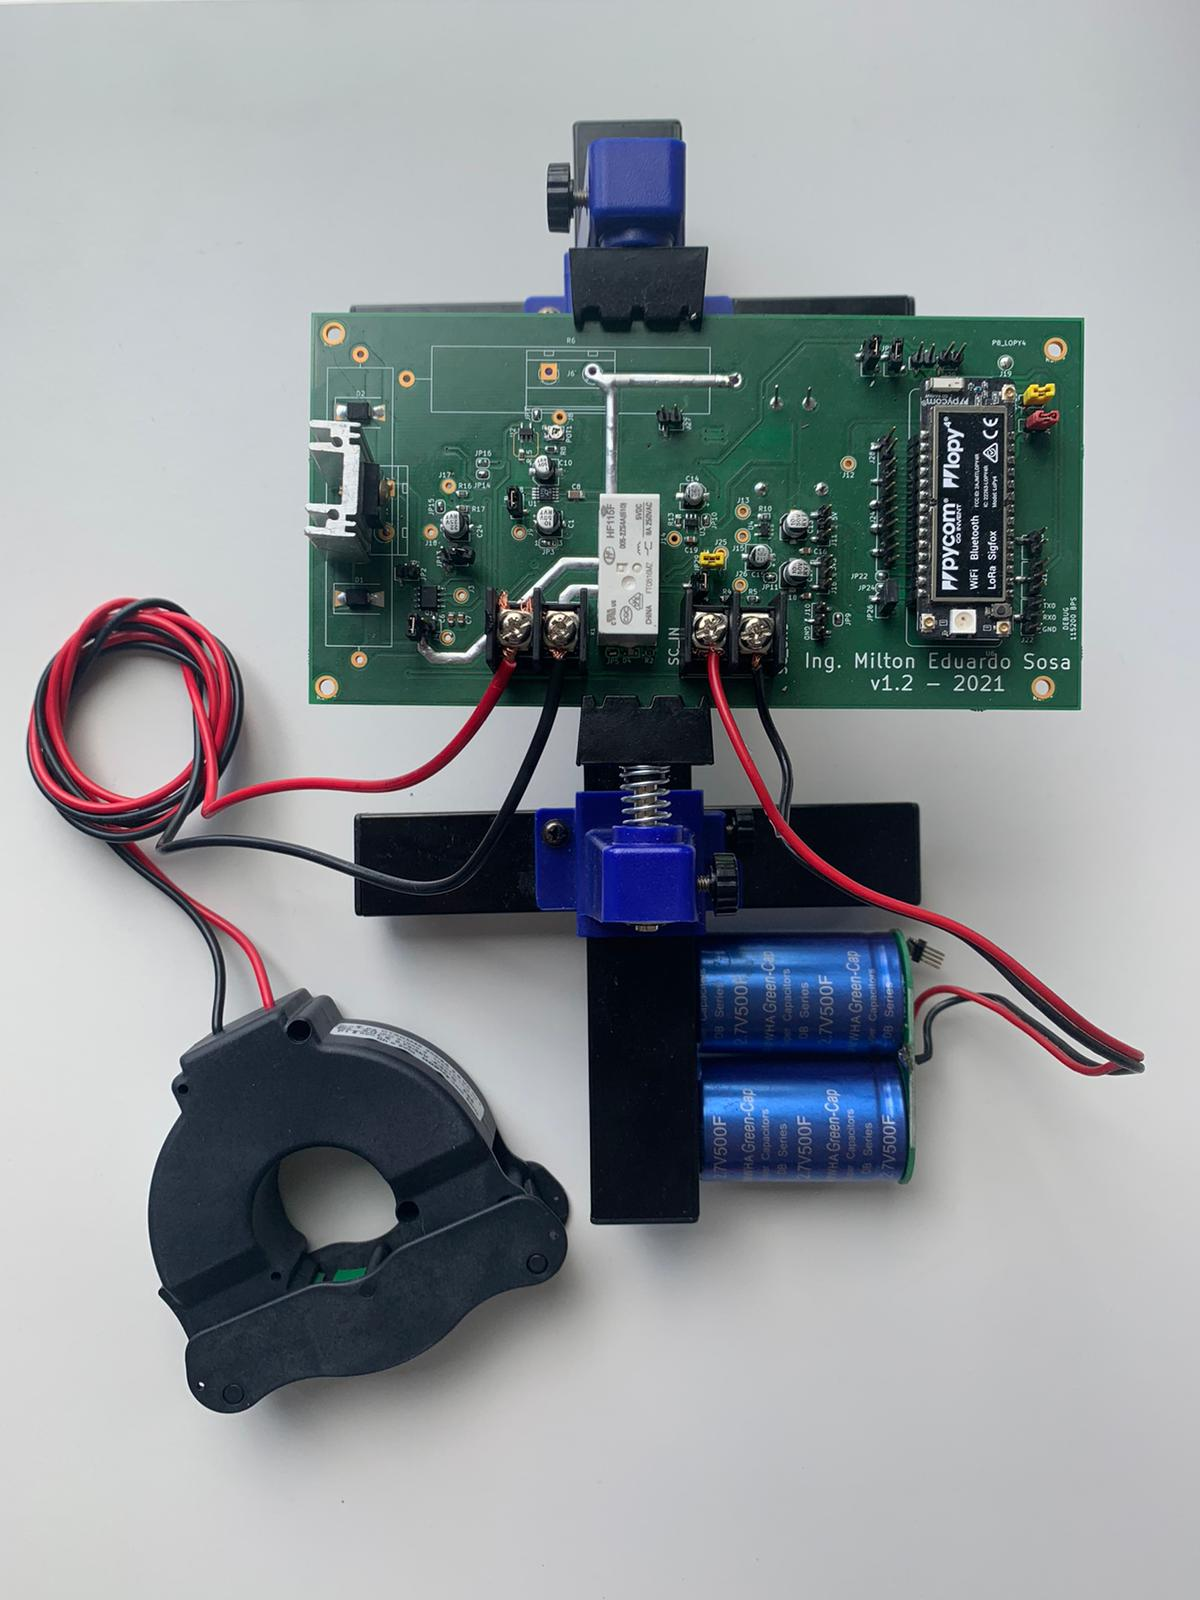
\includegraphics[width=1.0\linewidth]{Figures/banco_prueba_e2e_2}
	\caption{Lado TOP del circuito impreso final integrando todas las etapas.}
	\label{fig:pcbfinaltop}
\end{figure}\\
% TODO: \usepackage{graphicx} required
\begin{figure}[h!]
	\centering
	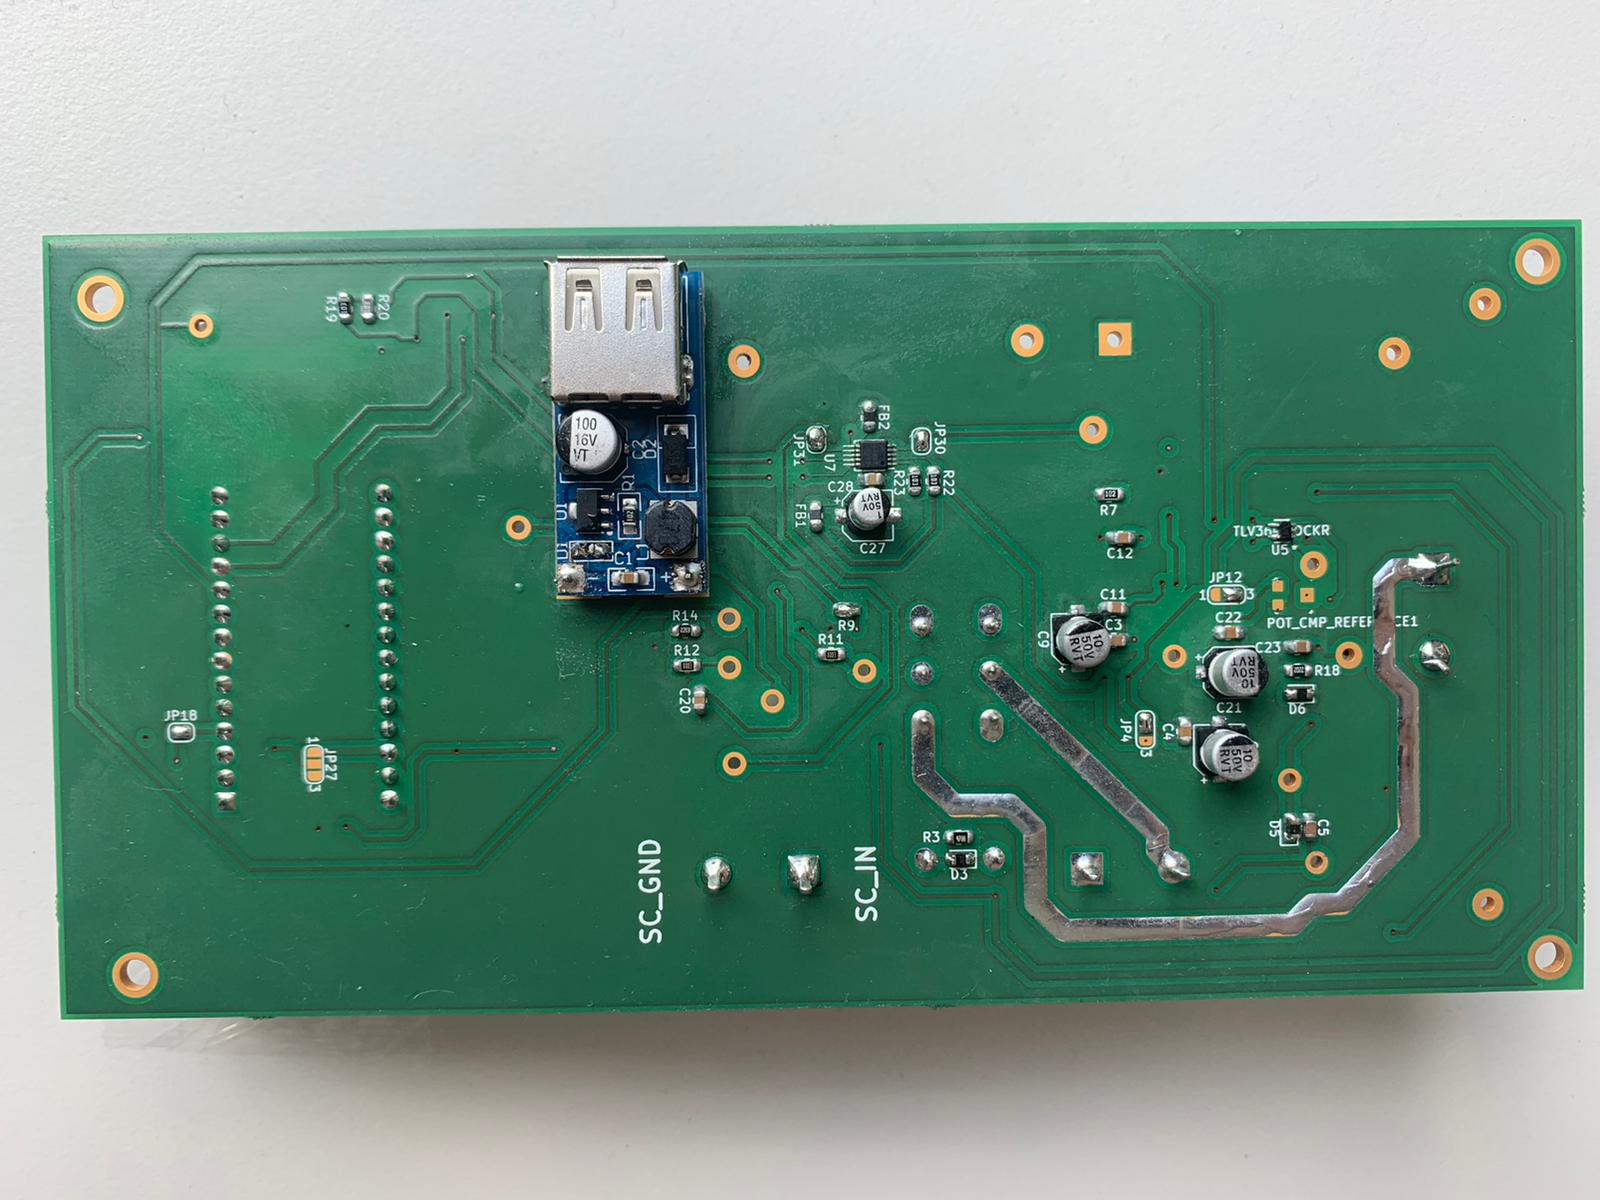
\includegraphics[width=1.0\linewidth]{Figures/pcb_fina_bottom}
	\caption{Lado BOTTOM del circuito impreso final que alberga todas las etapas.}
	\label{fig:pcbfinabottom}
\end{figure}

\section{Ensayos de laboratorio}
Debido a la imposibilidad de acceder a un laboratorio con instrumental de precisión, las mediciones tomadas en los ensayos se realizaron por partes y en diferentes turnos.\\
Como instrumento de medición se contó únicamente con un multímetro de la marca \textit{Hold Peak} modelo HP-770d \citep{hp770d}.\\
Un generador de señales de la marca \textit{Feel Tech} modelo FY6900 se empleó para inyectar una señal de 1 Vpp que simula la señal de tensión generada en bornes del shunt.
\subsection{Consumo en modo ahorro de energía o \textit{deep sleep}}
El mult\'{i}metro elegido tiene un rango que permite medir corriente desde los uA hasta 400 mA. Este rango resultó suficiente para la medición de corriente en ambos estados y evitar errores asociados al cambio de escala en el instrumento. Sin embargo, en las primeras rondas de medición se advirtió que al salir del modo ahorro de energía y transmitir, la corriente consumida por el hardware generó una tensión de burden en el instrumento que causó que el microcontrolador se reseteara por desvanecimiento (BOR, \textit{Brown Out Reset}-).\\
Como solución para el ensayo de consumo en \textit{deep sleep}, se grabó sobre la LoPy4 una versión de firmware que ni bien arranca, configura al hardware en modo ahorro de energía por 10 minutos. Este tiempo fue suficiente para registrar el consumo de corriente en este modo.\\
Para la medición de consumo durante la transmisión, se programó la versión final de firmware. Para sortear el problema de reseteo por desvanecimiento se utilizó la escala en amperes en conjunto con la función que retiene el pico máximo de la señal.\\
La tabla \ref{tabla_consumos} expone los resultados promediados para un total de 10 mediciones efectuadas en cada modo.\\
% \usepackage{color}
\begin{table}[h]
	\centering
	\caption{Consumo máximo registrado en los diferentes modos.}
	\begin{tabular}{cc} 
		\hline
		Modo                                                & \begin{tabular}[c]{@{}c@{}}Consumo\\\textcolor[rgb]{0.302,0.318,0.337}{máximo}\end{tabular}  \\ 
		\hline
		\begin{tabular}[c]{@{}c@{}}Deep\\sleep\end{tabular} & 62 uA                                                                                        \\
		Transmisión                                         & 127 mA                                                                                       \\
		\hline
	\end{tabular}\label{tabla_consumos}
\end{table}\\
Si bien el perfil estimado de consumo del hardware es similar al presentado en la figura \ref{fig:ciclodeepsleep}, por falta de equipamiento no se pudo capturar un oscilograma para graficar su perfil exacto.\\
Desenergizar toda la electrónica salvo al microcontrolador, ha reducido el consumo total de la electrónica al orden de los uA. Este valor de consumo registrado, se encuentra debajo de lo requerido por el cliente en \ref{req_deep_sleep} y se traduce en un aumento de la autonomía del acumulador.\\


\subsection{Autonom\'{i}a del supercapacitor}\label{ensayo_autonomia}
Este ensayo tuvo como objetivo principal, verificar el cumplimiento del requerimiento \ref{req_autonomia}.\\
Como única condición inicial, se adoptó que el supercapacitor esté cargado al máximo. Para acelerar el proceso, se lo cargó hasta una tensi\'{o}n de 4,67 V mediante una batería de 9 V convencional.\\
Como método de control y registro, se utilizó la tabla de base de datos \ref{tablacorrientesporfase}. El valor de tensión en bornes del supercapacitor se monitoreó de manera constante y se consideró como finalizada la prueba cuando se registró un cese en el almacenamiento de nuevos valores del nodo utilizado.\\
Con un tiempo de ahorro de energía de 5 minutos luego de transmitir, el hardware registr\'{o} una autonomía de 19 horas. Este valor resulta ser un 60\% mayor que el requerido por el cliente. Se estima que este valor podría aumentarse aún más anulando el indicador LED de encendido del relay, y/o proponiendo un circuito de selección de modo basado en un arreglo de transistores.\\

\subsection{Medidor de valor RMS}\label{ensayo_medidor_rms}
En este ensayo se analiz\'{o} la linealidad del circuito medidor de valor RMS implementado en la secci\'{o}n \ref{circuito_rms}.\\
El generador FY6900, simul\'{o} el valor de la señal generada en bornes del resistor shunt sin la necesidad de utilizar el transformador de corriente ni la carga.\\
Se realiz\'{o} un barrido de 10 pasos en la amplitud de la onda senoidal a la salida del generador. Simultáneamente, se registraron las tensiones RMS a la entrada del LTC1966 y a la salida de la etapa de amplificaci\'{o}n mediante el mult\'{i}metro. Los valores registrados, se exponen en la tabla \ref{tabla_ensayo_medidor_RMS} y a partir de estos se traz\'{o} la curva presentada en la figura \ref{fig:ensayoinealidadmedidorrms}.\\
Como se puede observar, la traza expone linealidad en todo el rango de medición del circuito implementado.\\
El error relativo resultó aceptable en m\'{a}s del 50 \% del rango de medición.\\
\begin{table}[h!]
	\centering
	\caption{Valores registrados en el ensayo de medici\'{o}n de valor RMS.}
	\begin{tabular}{ccccc} 
		\hline
		\begin{tabular}[c]{@{}c@{}}Vrms \\(V)\end{tabular} & \begin{tabular}[c]{@{}c@{}}Vout \\(V)\end{tabular} & \begin{tabular}[c]{@{}c@{}}Vout \\Esperado\\(V)\end{tabular} & \begin{tabular}[c]{@{}c@{}}error\\absoluto\\(mV)\end{tabular} & \begin{tabular}[c]{@{}c@{}}error relativo\\\%\end{tabular}  \\ 
		\hline
		0                                                  & 0,0520                                             & 0                                                            & 0,0520                                                        & -                                                           \\
		0,0323                                             & 0,3260                                             & 0,3034                                                       & 0,0226                                                        & 7,44                                                        \\
		0,0690                                             & 0,6650                                             & 0,6476                                                       & 0,0174                                                        & 2,69                                                        \\
		0,1059                                             & 1,0050                                             & 0,9945                                                       & 0,0105                                                        & 1,06                                                        \\
		0,1434                                             & 1,3500                                             & 1,3467                                                       & 0,0033                                                        & 0,25                                                        \\
		0,1811                                             & 1,6960                                             & 1,7007                                                       & 0,0047                                                        & 0,28                                                        \\
		0,2109                                             & 1,9690                                             & 1,9806                                                       & 0,0116                                                        & 0,58                                                        \\
		0,2479                                             & 2,3090                                             & 2,3280                                                       & 0,0190                                                        & 0,82                                                        \\
		0,2819                                             & 2,6220                                             & 2,6473                                                       & 0,0253                                                        & 0,96                                                        \\
		0,3193                                             & 2,974                                              & 2,9985                                                       & 0,0245                                                        & 0,82                                                        \\
		0,3535                                             & 3,313                                              & 3,3197                                                       & 0,0067                                                        & 0,20                                                        \\
		\hline
	\end{tabular}\label{tabla_ensayo_medidor_RMS}
\end{table}
% TODO: \usepackage{graphicx} required
\begin{figure}[h!]
	\centering
	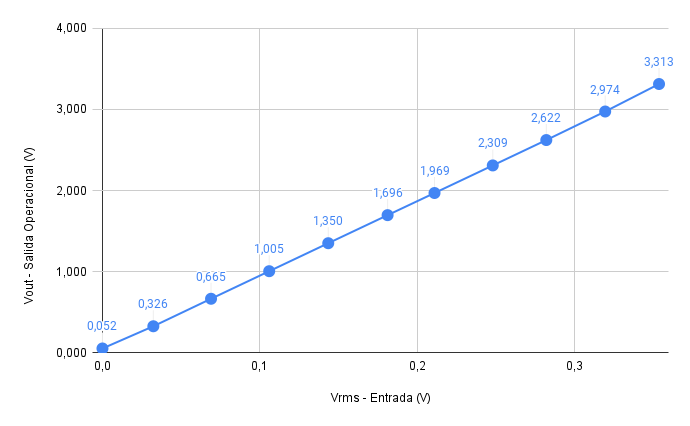
\includegraphics[width=1.0\linewidth]{Figures/ensayo_inealidad_medidor_RMS}
	\caption{Traza para análisis de linealidad del medidor de valor RMS.}
	\label{fig:ensayoinealidadmedidorrms}
\end{figure}\\
\vspace{200px}
\subsection{Detecci\'{o}n de cortes}
Este ensayo tuvo por objeto verificar el correcto funcionamiento del circuito de la figura \ref{fig:ctodetectorcortes}, encargado de detectar la interrupci\'{o}n en el servicio de distribuci\'{o}n de energía el\'{e}ctrica y generar una interrupci\'{o}n por hardware.\\
Como condici\'{o}n inicial se carg\'{o} el banco de supercapacitores hasta una tensión cercana a 5 V. 
El banco de pruebas de la figura \ref{fig:bancopruebae2e2} est\'{a} compuesto por una estufa que consume 13 A y un tomacorrientes que se utiliz\'{o} para simular la red de distribuci\'{o}n de energía el\'{e}ctrica y sus posibles interrupciones en el suministro.\\
% TODO: \usepackage{graphicx} required
\begin{figure}[h]
	\centering
	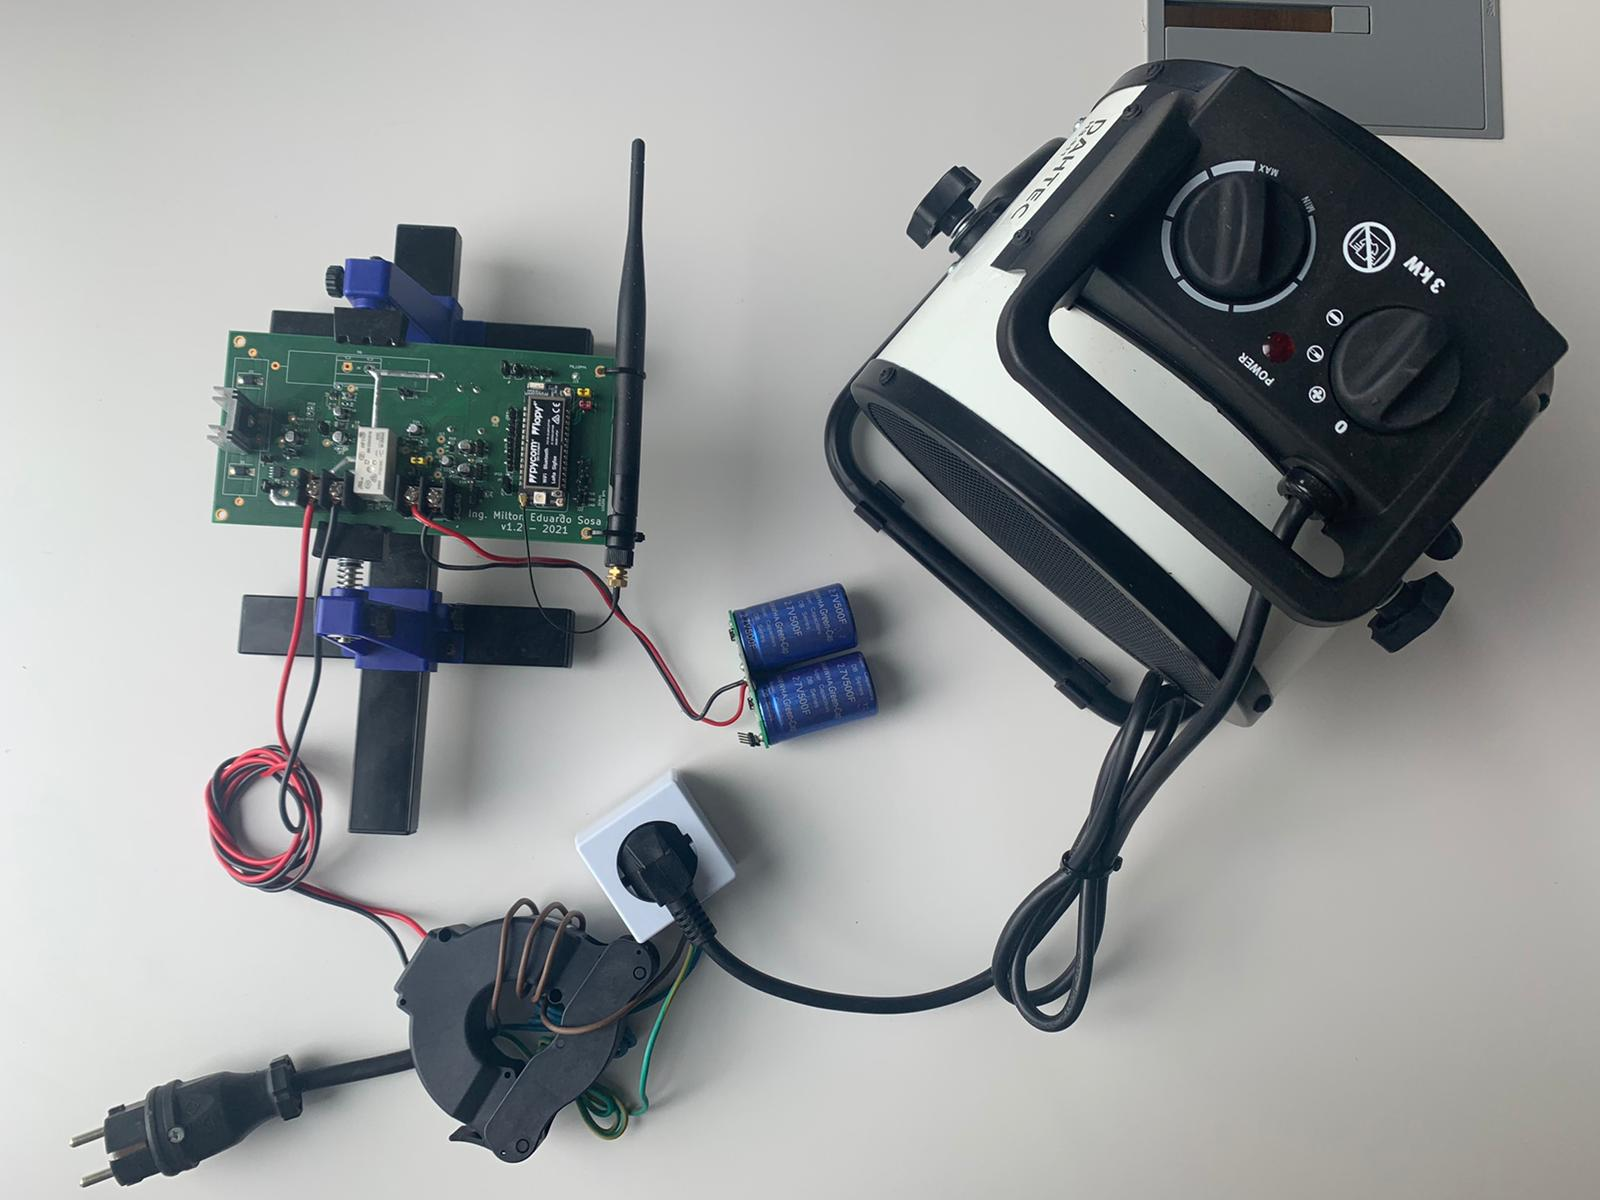
\includegraphics[width=1.0\linewidth]{Figures/banco_prueba_e2e_1}
	\caption{Banco de prueba utilizado en ensayos del circuito detector de corte y end-to-end.}
	\label{fig:bancopruebae2e2}
\end{figure}\\
Para simular diferentes pasos de corrientes a trav\'{e}s del transformador de intensidad, se increment\'{o} el n\'{u}mero de vueltas en el devanado primario. De esta manera se aument\'{o} proporcionalmente el flujo magn\'{e}tico encauzado por el transformador de intensidad, sin aumentar la carga a la que se someti\'{o} la red el\'{e}ctrica del banco de prueba.\\
Los resultados demostraron que una corriente en el primario por debajo de los 50 A, genera una interrupci\'{o}n por hardware exitosamente. El microcontrolador sali\'{o} del modo ahorro de energía y envi\'{o} de manera correcta un reporte de estado indicando una lectura de 0 A a los servicios de backend.\\
Una demostraci\'{o}n del funcionamiento de esta etapa ante el cliente dió por finalizado este ensayo de manera exitosa.\\

\section{Ensayos \textit{end to end}}
Con objeto de realizar una prueba final de integraci\'{o}n y funcionamiento de todas las partes, se decidi\'{o} repetir los ensayos descritos en \ref{ensayo_autonomia} y \ref{ensayo_medidor_rms}. Para los ensayos \textit{end to end} se utilizaron los paneles de Grafana para la visualización de los datos. De este modo, se comtempló el funcionamiento de todos los módulos de hardware y software desarrollados para este proyecto, lográndose la verificación del cumplimiento de los objetivos generales.\\
Es importante mencionar que, si bien el autor cont\'{o} físicamente con el hardware en todo momento, no fue as\'{i} con los servicios de backend. Estos corrieron en todo momento sobre una Raspberry Pi 3 B+ localizada en la provincia de Misiones desde el principio del proyecto.\\
Los resultados del ensayo de autonomía expuestos en la figura \ref{fig:e2esupercap}, demuestran el correcto funcionamiento y despliegue de informaci\'{o}n hist\'{o}rica de la tensión en bornes del supercapacitor.\\
% TODO: \usepackage{graphicx} required
\begin{figure}[h]
	\centering
	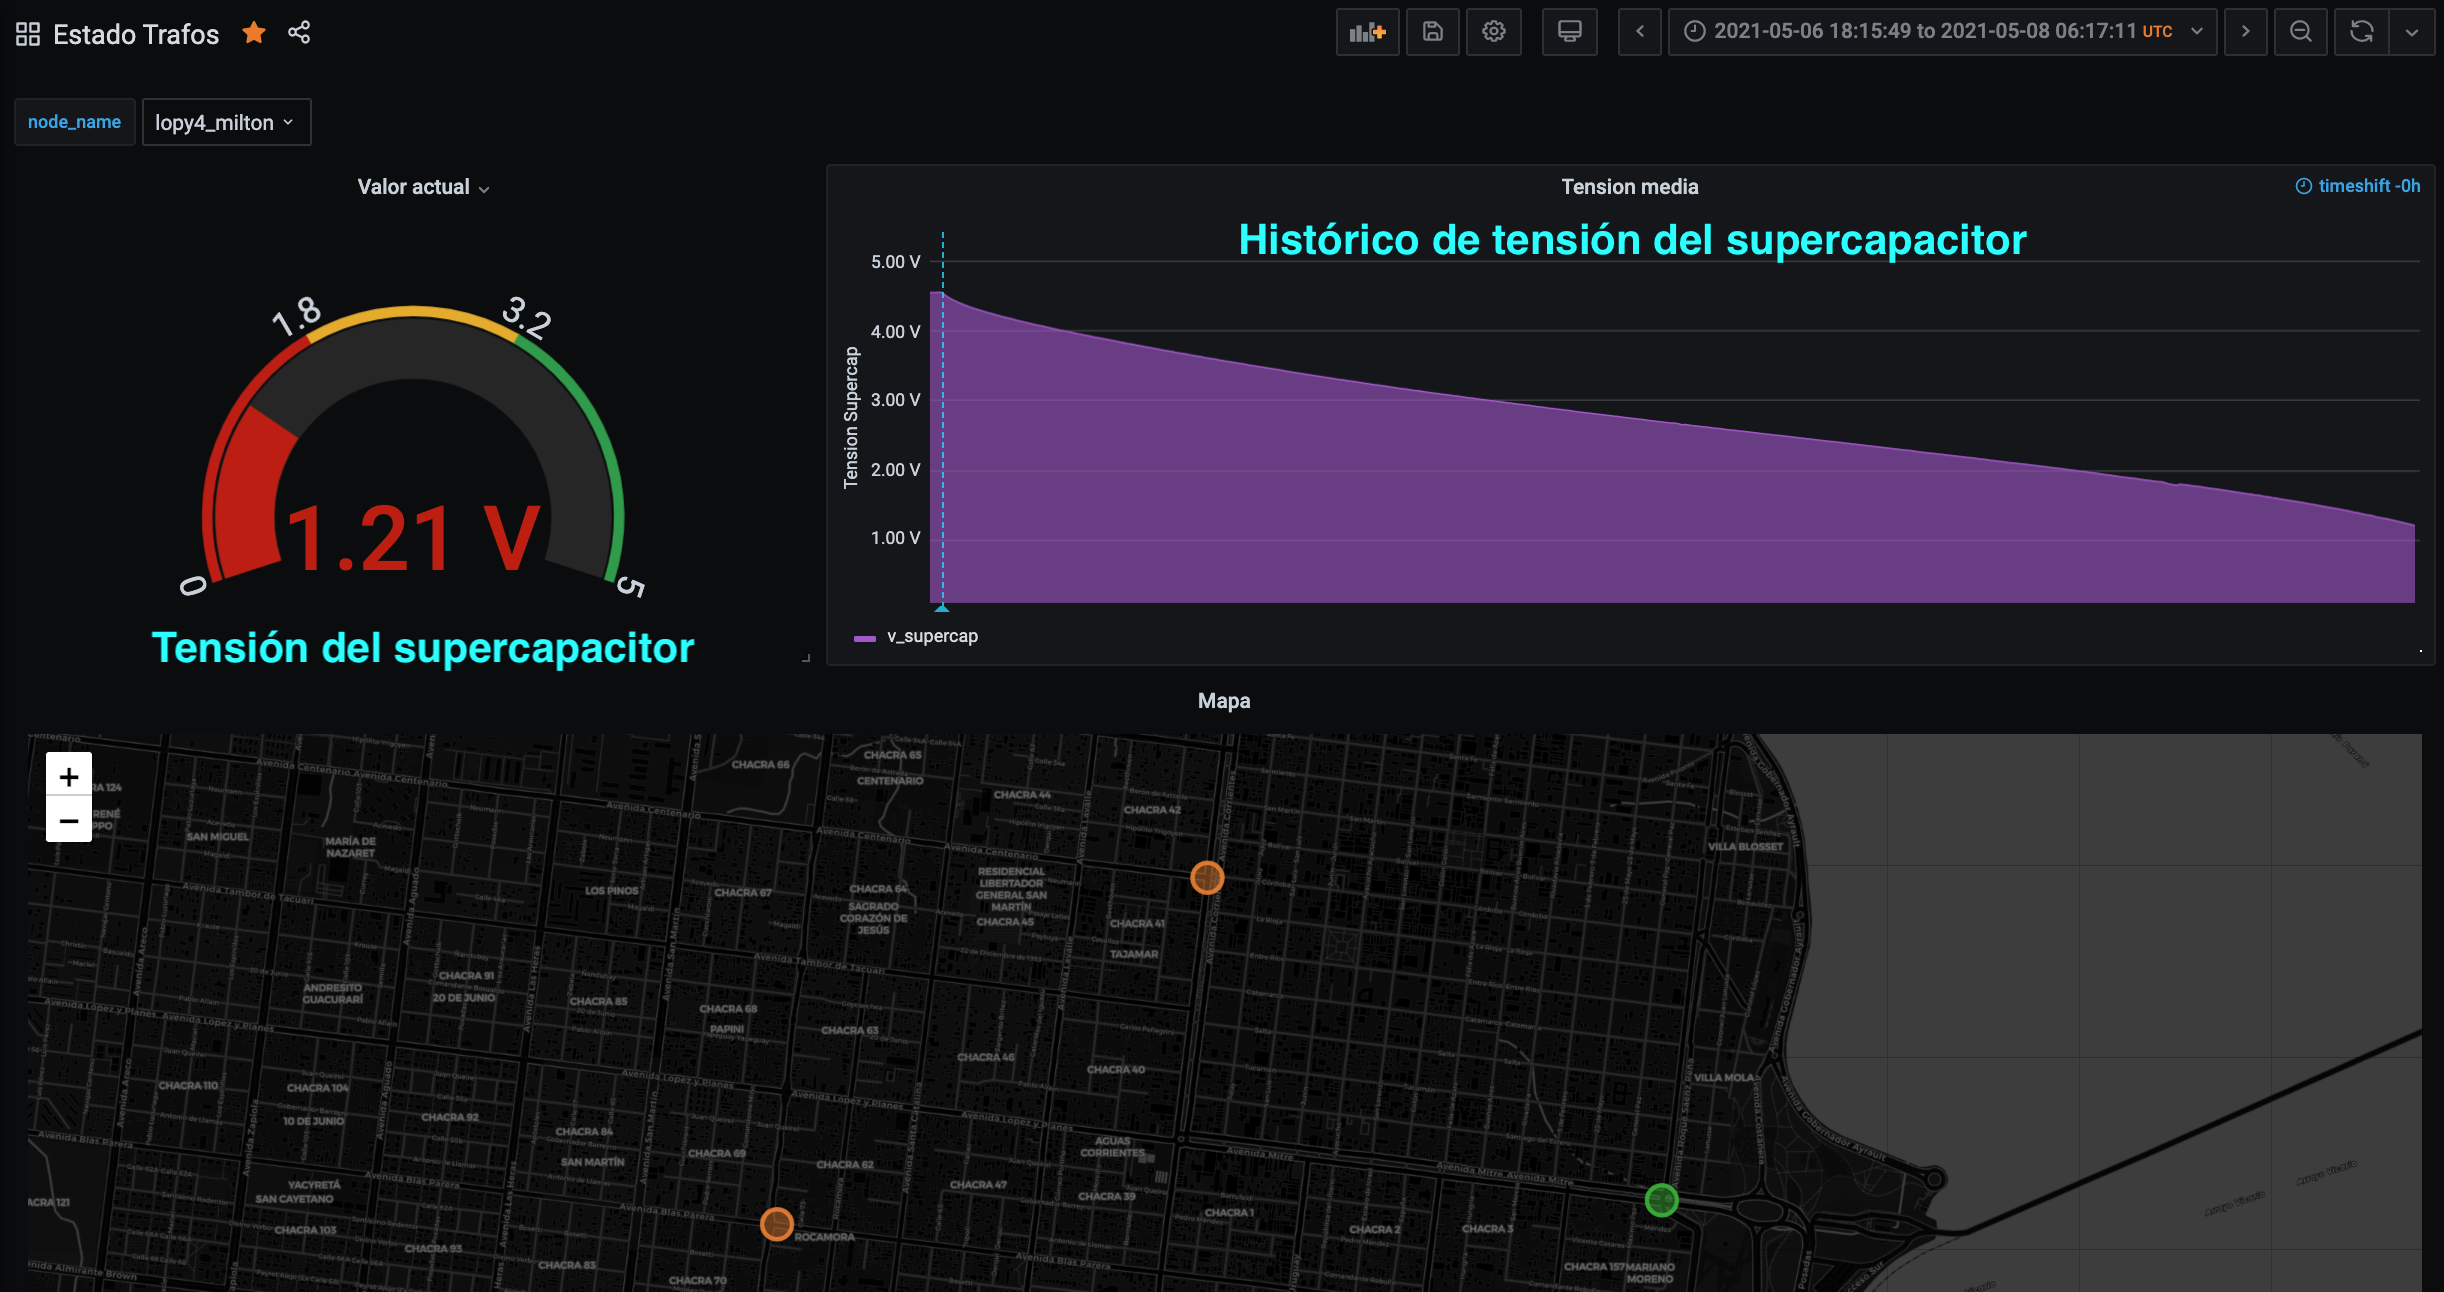
\includegraphics[width=1.0\linewidth]{Figures/e2e_supercap}
	\caption{Ensayo end to end de autonom\'{i}a.}
	\label{fig:e2esupercap}
\end{figure}\\
Por su parte en el ensayo de medici\'{o}n de corriente de la figura \ref{fig:capturahistoricodropdown}, se expone correctamente la evoluci\'{o}n de la corriente medida por el circuito expuesto en \ref{circuito_rms}.\\
El agregado de un \textit{drop down menu} en ambos paneles, permite rápidamente elegir de qu\'{e} nodo de la flota se desea ver la informaci\'{o}n a desplegar en las trazas.\\
Por \'{u}ltimo, con respecto a la rapidez de propagaci\'{o}n de los datos desde que son generados por el hardware hasta aparecer en la interfaz gráfica de usuario, el tiempo promedio fue de 5 a 7 segundos. Una nueva demostraci\'{o}n ante el cliente di\'{o} por finalizada la prueba satisfactoriamente.
\vspace{200px}
% TODO: \usepackage{graphicx} required
\begin{figure}[h!]
	\centering
	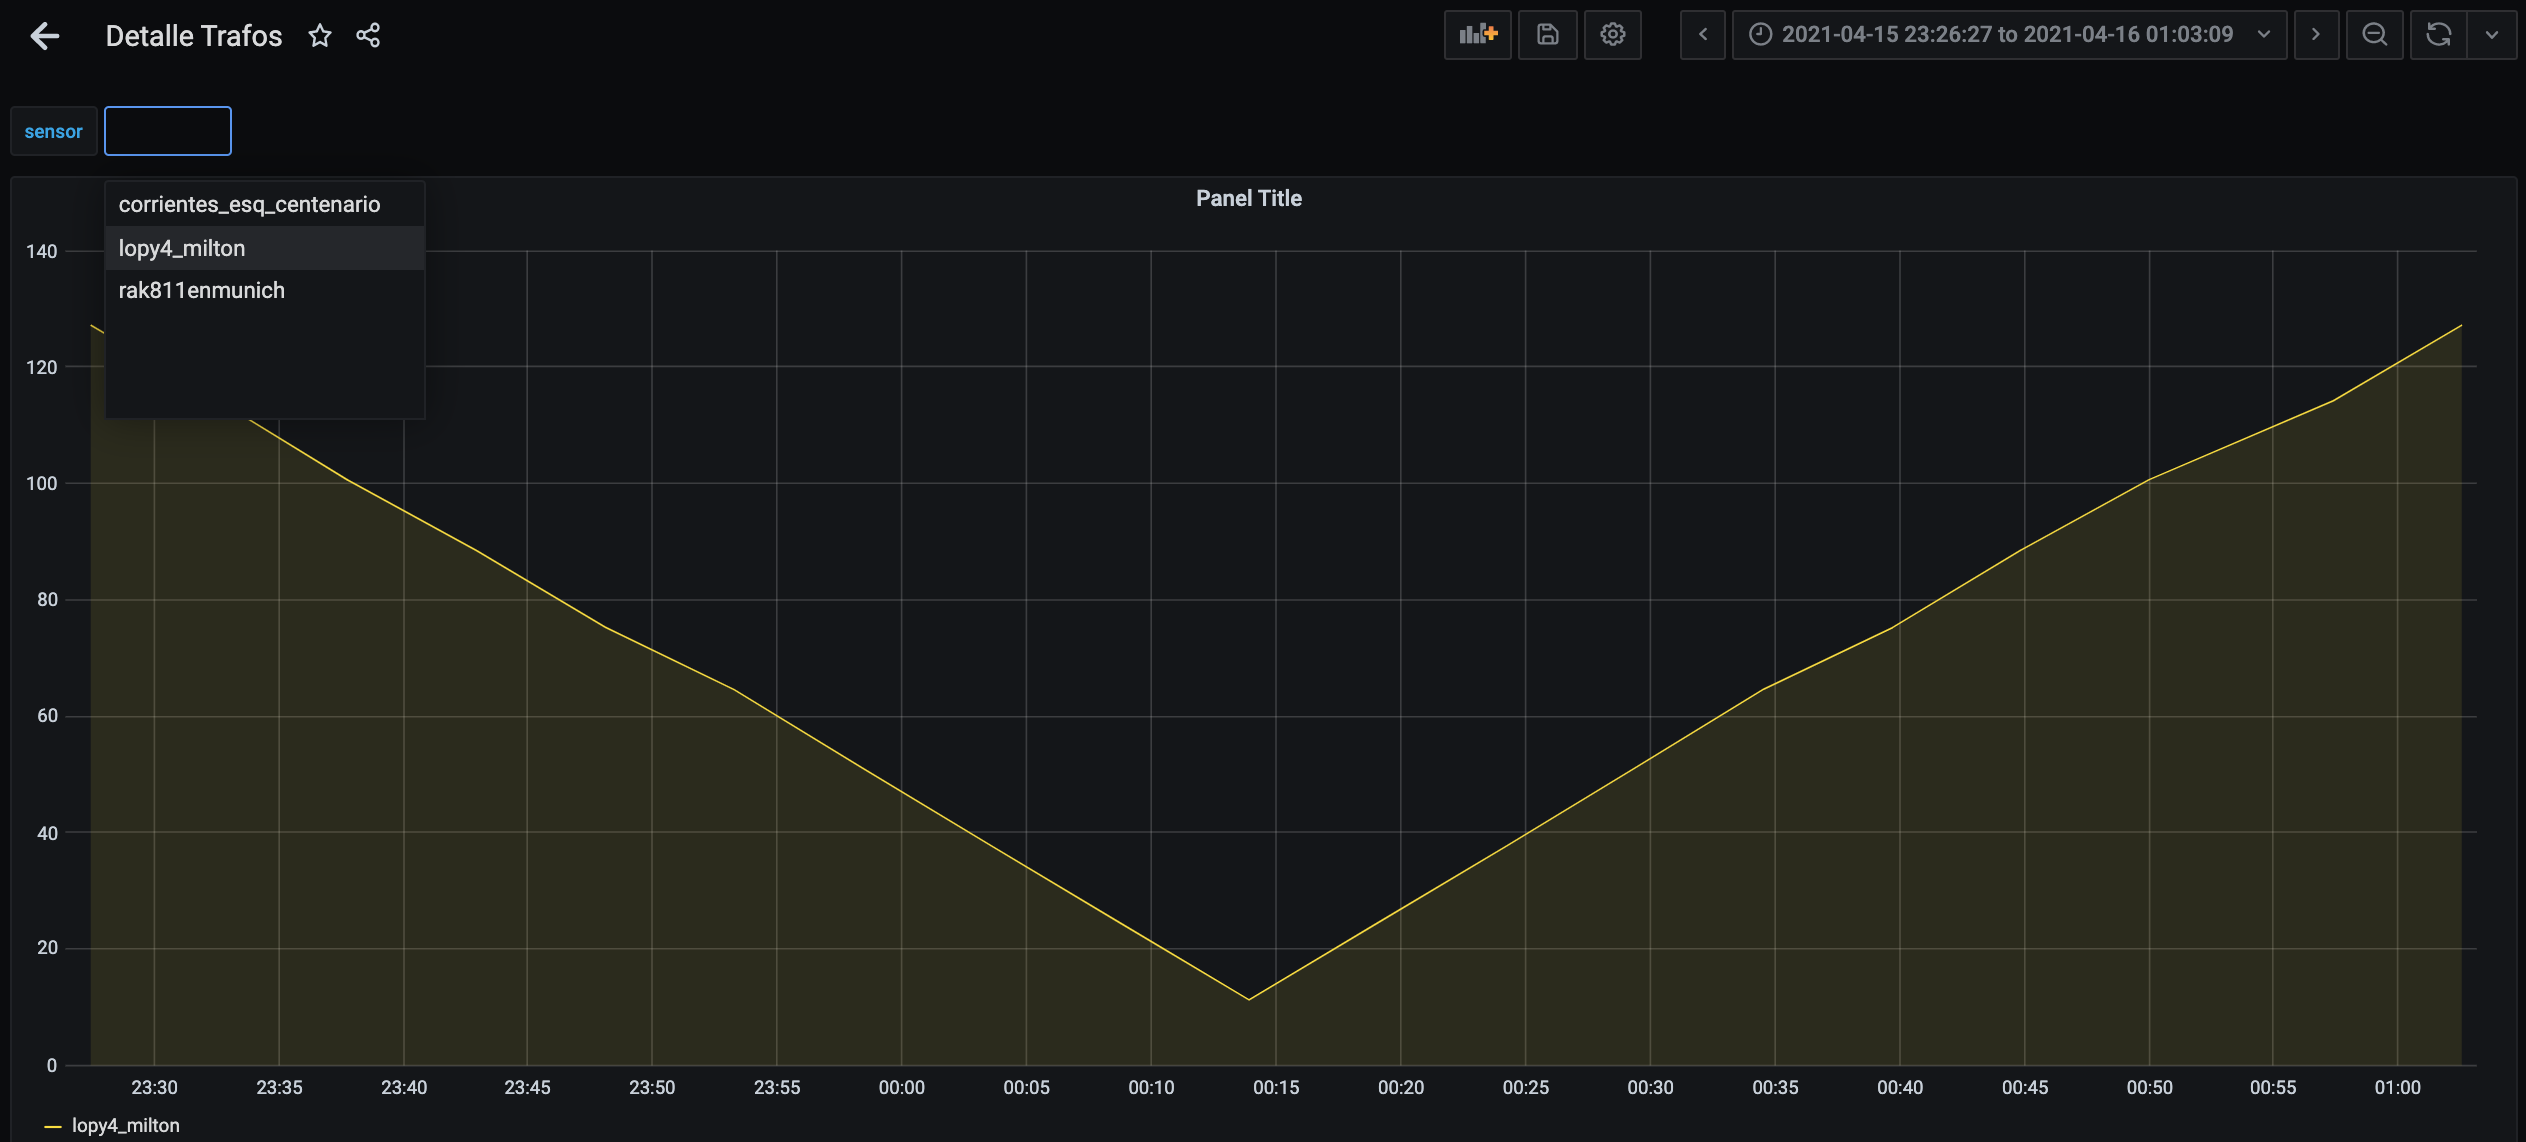
\includegraphics[width=1.0\linewidth]{Figures/captura_historico_dropdown}
	\caption{Ensayo end-to-end de medici\'{o}n de corriente.}
	\label{fig:capturahistoricodropdown}
\end{figure}\\